\subsubsection{27.12.14}
\begin{enumerate}
	
	\item Время начала и окончания собрания: 1:00 - 2:00.
	
	\item Цели собрания: 
	\begin{enumerate}
		
		\item Закончить облуживание проводов.
		
		\item Разработать механизм, позволяющий МЗК удерживать подвижную корзину после отключения питания.
		
        \item Реализовать более удобную программу управления движением робота.
		
	\end{enumerate}

	\item Проделанная работа:
	\begin{enumerate}
		
		\item Все провода были залужены.
		
		\item Для того, чтобы МЗК не открывался под тяжестью корзины (в том случае, когда робот завозит ее на пандус) после отключения питания, было решено установить на него две пары одежных липучек, достаточно слабых, чтобы препятствовать работе сервопривода, приводящего в движение МЗК, но достаточно сильных, чтобы удержать корзину. Липучки были установлены, но испытать усовершенствование не получилось, поскольку у нас нет в распоряжении оригинальных подвижных корзин.
		
		\begin{figure}[H]
			\begin{minipage}[h]{0.1\linewidth}
				\center  
			\end{minipage}
			\hfill
			\begin{minipage}[h]{0.29\linewidth}
				\center{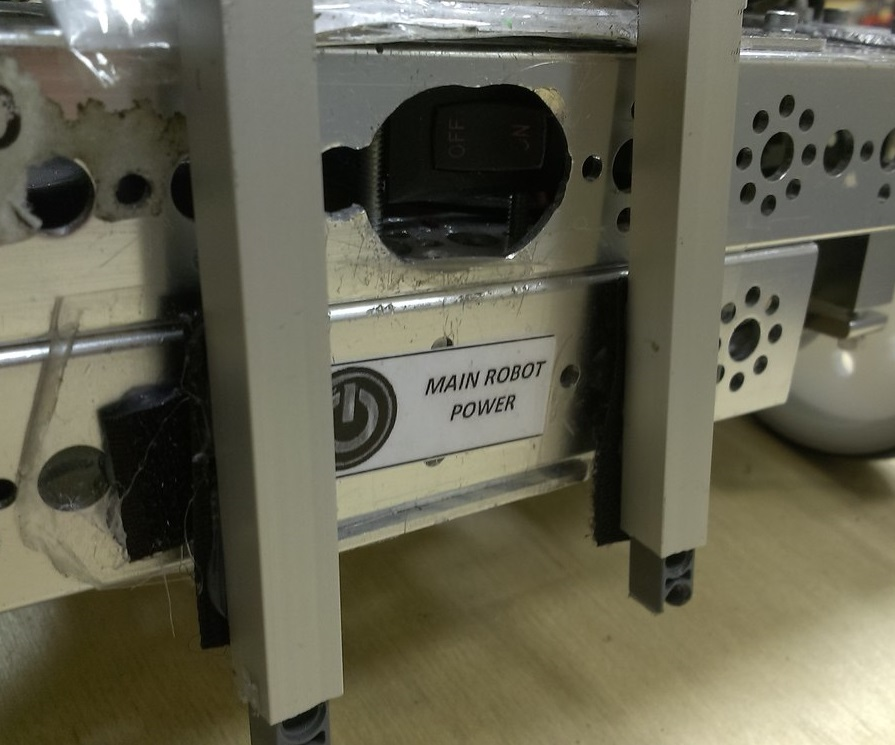
\includegraphics[scale=0.2]{days/27.12.14/images/01}}
			\end{minipage}
			\hfill
			\begin{minipage}[h]{0.29\linewidth}
				\center{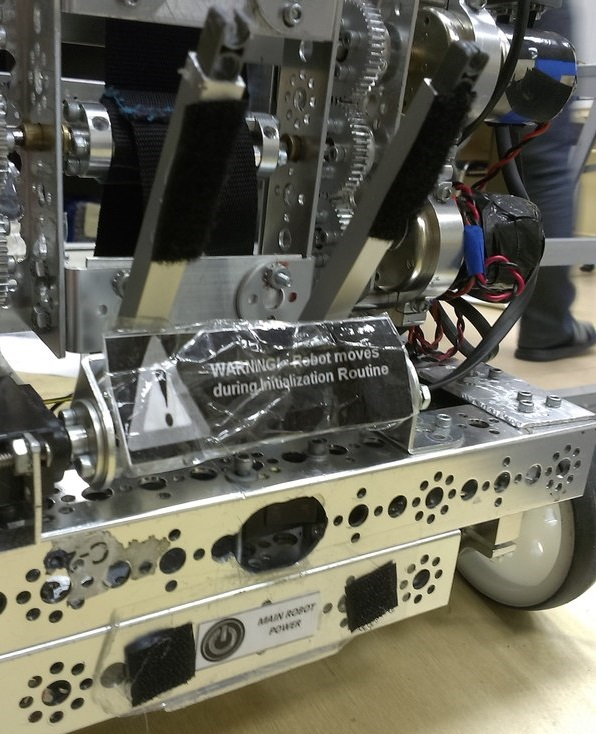
\includegraphics[scale=0.2]{days/27.12.14/images/02}}
			\end{minipage}
			\hfill
			\begin{minipage}[h]{0.1\linewidth}
				\center  
			\end{minipage}
			\caption{Липучки на МЗК}
		\end{figure}
		
        \item Была реализована более удобная программа управления движением робота. Управление движением с левого аналогового датчика (стика) было перенесено на многопозиционную кнопку "TopHat". Так, теперь можно задать роботу двигаться восемью способами: Вперед, назад, танковый разворот вокруг своей оси по часовой стрелке и против, а также вращение только одной парой приводов (левой или правой) вперед или назад, в результате чего получается разворот вокруг неподвижной пары приводов. Кроме того, при удержании кнопок 6 или 7 включается медленное движение.
		
        \begin{figure}[H]
	  	  \begin{minipage}[h]{0.2\linewidth}
	  		\center  
	  	  \end{minipage}
	  	  \begin{minipage}[h]{0.6\linewidth}
	  		\center{
\includegraphics[scale=0.3]{days/27.12.14/images/03}}
	  		\caption{Схема управления движением}
	  	  \end{minipage}
	   \end{figure}
	   
	   \item Во время испытания программы движения было замечено, что замененный ранее привод (правый задний) не работает на поле (он прокручивается без нагрузки, когда робот находится на весу, но когда робот стоит на поле, этом привод не способен сдвинуть его с места). Несмотря на это, робот выполнял хорошо 5 из 8 команд (движение по прямой, разворот по часовой стрелке, развороты с использованием только левой парой колес). Опытным путем удалось выяснить, что неисправен именно привод, а не драйвер приводов. Необходимо снова заменить привод для того, чтобы робот мог нормально выполнять все возможные виды движения.
	   
	\end{enumerate}
	
	\item Итоги собрания:
	\begin{enumerate}
		
		\item Все провода залужены.
		
		\item МЗК усовершенствован, но не испытан.
		
        \item Новая программа движения написана и протестирована. Результат положительный.
		
	\end{enumerate}
	
	\item Задачи для последующих собраний:
	\begin{enumerate}
		
		\item Заменить сломанный привод.
		
		\item Заменить сломанную рейку подъемника.
			
	\end{enumerate}
\end{enumerate}
\fillpage
